\section{Ti\textit{k}Z package}

\begin{quote}
    2020-05-01: first update
\end{quote}

%%%%%%%%%%%%%%%%%%%%%%%%%%%%%%%%%%%%%%%%%%%%
%%%%%%%%%%%%%%%%%%%%%%%%%%%%%%%%%%%%%%%%%%%%

\subsection{Package settings}

\begin{enumerate}
    \item TikZ library

\begin{lstlisting}[language=Tex]
\usepackage{tikz}
\usetikzlibrary{shapes.geometric, arrows}
\end{lstlisting}

For more details, please refer to \href{https://tex.stackexchange.com/questions/42611/list-of-available-tikz-libraries-with-a-short-introduction}{List of available TikZ libraries with a short introduction - stackexchange}.

\item \texttt{tikzstyle}

Theis command could be used to define the basic components of a flowchart, which is discussed in detail in Section~\ref{subsub:flowchart}.

\end{enumerate}

%%%%%%%%%%%%%%%%%%%%%%%%%%%%%%%%%%%%%%%%%%%%
%%%%%%%%%%%%%%%%%%%%%%%%%%%%%%%%%%%%%%%%%%%%

\subsection{Examples}

\subsubsection{Basic shapes}

\begin{enumerate}

\item drawing a square
    
\begin{lstlisting}[language=Tex]
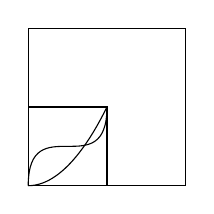
\begin{tikzpicture}
    %% line
    \draw (0,0) -- (0,2) -- (2,2) -- (2,0) -- (0,0);
    % end in the start to form a cycle
    \draw (0,0) -- (0,2) -- (2,2) -- (2,0) -- cycle;
    % use the rectangle keyword to simplify
    \draw (0,0) rectangle (1,1);
    %% parabola
    \draw (0,0) parabola (1,1);
    % add control points
    \draw (0,0) .. controls (0,1) and (1,0) .. (1,1);
\end{tikzpicture}
\end{lstlisting}

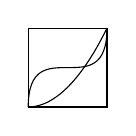
\begin{tikzpicture}
    %\draw (0,0) -- (0,2) -- (2,2) -- (2,0) -- (0,0);
    %\draw (0,0) -- (0,2) -- (2,2) -- (2,0) -- cycle;
    \draw (0,0) rectangle (1,1);
    \draw (0,0) parabola (1,1);
    \draw (0,0) .. controls (0,1) and (1,0) .. (1,1);
\end{tikzpicture}

\item draw a circle/ellipse/arc with line style

\begin{lstlisting}[language=Tex]
\begin{tikzpicture}
     % center and radius
    \draw (1,1) circle (1cm);
    \draw (2,1) circle (0.5cm);
    % center and semi-axis in x/y
    \draw (2,1) ellipse (1cm and 0.5cm);
    % start point and (start:end:radius)
    \draw (2,1) arc (0:30:2cm)
    % line style
    \draw[red,thick,dashed] (1,1) circle (0.5cm);
\end{tikzpicture}
\end{lstlisting}

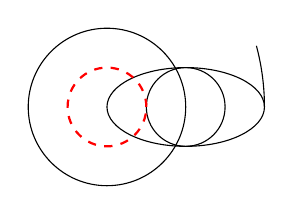
\begin{tikzpicture}
    \draw (1,1) circle (1cm);
    \draw (2,1) circle (0.5cm);
    \draw (2,1) ellipse (1cm and 0.5cm);
    \draw (3,1) arc (0:15:3cm);
    \draw[red,thick,dashed] (1,1) circle (0.5cm);
\end{tikzpicture}
    
\item Grids with filling

\begin{lstlisting}
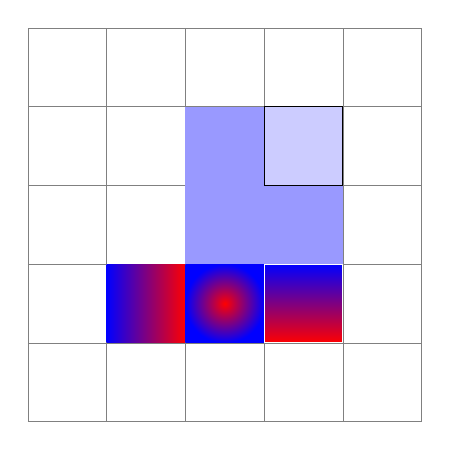
\begin{tikzpicture}
    %% grid
    % bottom-left -> top-right
    \draw[step=1cm,gray,very thin] (-2,-2) grid (3,3);
    %% color filling
    \fill[blue!40!white] (0,0) rectangle (2,2); % 40% blue mixed with 60% white
    %% fill with border
    \filldraw[blue!20!white, draw=black] (1,1) rectangle (2,2);
    %% fill with color gradient
    % left/right/top/bottom/inner/outer color
    \shade[left color=blue, right color=red] (-1,-1) rectangle (0,0);
    \shade[outer color=blue, inner color=red] (0,-1) rectangle (1,0);
    %% fill with color gradient and border
    \shadedraw[top color=blue,bottom color=red, draw=white] (1,-1) rectangle (2,0);
\end{tikzpicture}
\end{lstlisting}

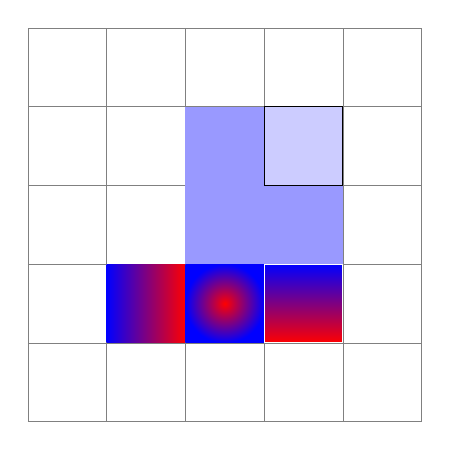
\begin{tikzpicture}
    \draw[step=1cm,gray,very thin] (-2,-2) grid (3,3);
    \fill[blue!40!white] (0,0) rectangle (2,2);
    \filldraw[blue!20!white, draw=black] (1,1) rectangle (2,2);
    \shade[left color=blue, right color=red] (-1,-1) rectangle (0,0);
    \shade[outer color=blue, inner color=red] (0,-1) rectangle (1,0);
    \shadedraw[top color=blue,bottom color=red, draw=white] (1,-1) rectangle (2,0);
\end{tikzpicture}

\item combining line and grid

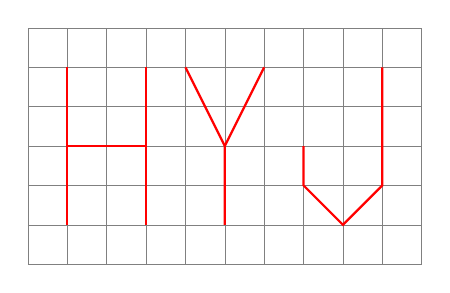
\begin{tikzpicture}
    \draw[step=0.5cm,gray,very thin] (0,0) grid (5,3);
    % H
    \draw[red,thick] (0.5,0.5) -- (0.5,2.5);
    \draw[red,thick] (0.5,1.5) -- (1.5,1.5);
    \draw[red,thick] (1.5,0.5) -- (1.5,2.5);
    % Y
    \draw[red,thick] (2.5,0.5) -- (2.5,1.5) -- (2,2.5);
    \draw[red,thick] (2.5,1.5) -- (3,2.5);
    % J
    \draw[red,thick] (3.5,1.5) -- (3.5,1) -- (4,0.5) -- (4.5,1) -- (4.5,2.5);
\end{tikzpicture}

\item Axes with text

\begin{lstlisting}
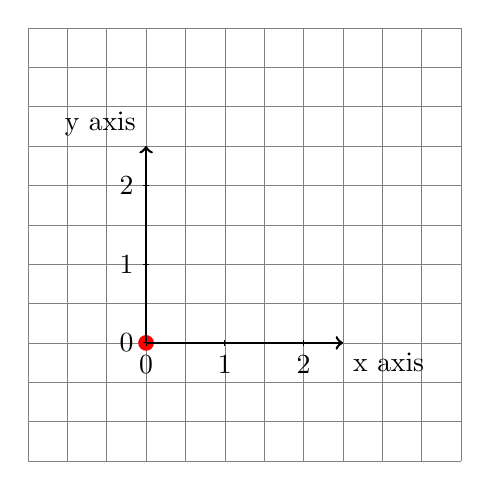
\begin{tikzpicture}
    %% grid
    \draw[step=0.5cm,gray,very thin] (-1.5,-1.5) grid (4,4);
    \fill[red] (0,0) circle (0.1cm);
    
    %% Axes
    \draw[thick,->] (0,0) -- (0,2.5);
    \draw[thick,->] (0,0) -- (2.5,0);
    
    % label our axes using nodes
    \draw[thick,->] (0,0) -- (2.5,0) node[anchor=north west] {x axis};
    \draw[thick,->] (0,0) -- (0,2.5) node[anchor=south east] {y axis};
    
    % add in ticks and numbering
    \foreach \x in {0,1,2}
        \draw (\x cm,1pt) -- (\x cm,-1pt) node[anchor=north] {$\x$};
    \foreach \y in {0,1,2}
        \draw (1pt,\y cm) -- (-1pt,\y cm) node[anchor=east] {$\y$};
\end{tikzpicture}
\end{lstlisting}

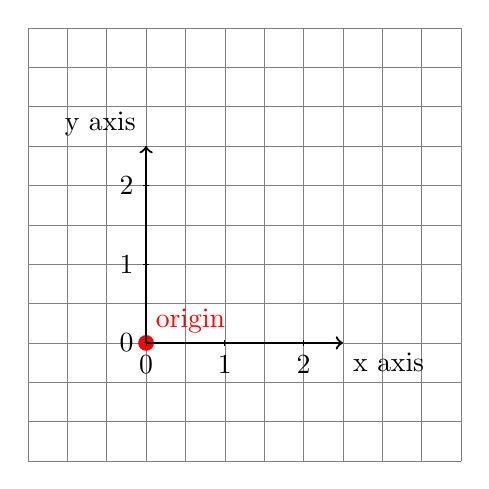
\begin{tikzpicture}
    \draw[step=0.5cm,gray,very thin] (-1.5,-1.5) grid (4,4);
    
    \fill[red] (0,0) circle (0.1cm) node[anchor=south west] {origin};
    \draw[thick,->] (0,0) -- (2.5,0) node[anchor=north west] {x axis};
    \draw[thick,->] (0,0) -- (0,2.5) node[anchor=south east] {y axis};
    
    \foreach \x in {0,1,2}
        \draw (\x cm,1pt) -- (\x cm,-1pt) node[anchor=north] {$\x$};
    \foreach \y in {0,1,2}
        \draw (1pt,\y cm) -- (-1pt,\y cm) node[anchor=east] {$\y$};
\end{tikzpicture}

\end{enumerate}

\subsubsection{Creating flowchart}
\label{subsub:flowchart}

\begin{enumerate}
    \item define block style
    
\begin{lstlisting}[language=Tex]
\tikzstyle{startstop} = [rectangle, rounded corners, minimum width=3cm, minimum height=1cm,text centered, draw=black, fill=red!30]
\tikzstyle{io} = [trapezium, trapezium left angle=70, trapezium right angle=110, minimum width=3cm, minimum height=1cm, text centered, draw=black, fill=blue!30]
\tikzstyle{process} = [rectangle, minimum width=3cm, minimum height=1cm, text centered, draw=black, fill=orange!30]
\tikzstyle{decision} = [diamond, minimum width=3cm, minimum height=1cm, text centered, draw=black, fill=green!30]
\tikzstyle{arrow} = [thick,->,>=stealth]
\end{lstlisting}

\item add nodes

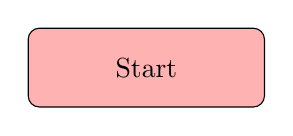
\begin{tikzpicture}[node distance=2cm]
\node (start) [startstop] {Start};
\end{tikzpicture}

\item connect with arrows

\hl{to be updated}

\end{enumerate}

\subsubsection{Creating TikZ from GeoGebra}

\hl{to be updated}

%%%%%%%%%%%%%%%%%%%%%%%%%%%%%%%%%%%%%%%%%%%%
%%%%%%%%%%%%%%%%%%%%%%%%%%%%%%%%%%%%%%%%%%%%

\subsection{Useful links}

\begin{enumerate}

    \item \href{https://mirror.foobar.to/CTAN/graphics/pgf/base/doc/pgfmanual.pdf}{The TikZ and PGF Packages}
    
        Manual for version 3.1.8b, December 27, 2020
    \item LaTeX Graphics using TikZ: A Tutorial for Beginners - Overleaf
    
    \href{https://www.overleaf.com/learn/latex/LaTeX_Graphics_using_TikZ:_A_Tutorial_for_Beginners_(Part_1)%E2%80%94Basic_Drawing}{Part 1-Basic Drawing}; 
    \href{https://www.overleaf.com/learn/latex/LaTeX_Graphics_using_TikZ:_A_Tutorial_for_Beginners_(Part_2)%E2%80%94Generating_TikZ_Code_from_GeoGebra}{Part 2-Generating TikZ Code from GeoGebra}; 
    \href{https://www.overleaf.com/learn/latex/LaTeX_Graphics_using_TikZ:_A_Tutorial_for_Beginners_(Part_3)%E2%80%94Creating_Flowcharts}{Part 3-Creating Flowcharts}
    
    \item \href{https://tex.stackexchange.com/questions/42611/list-of-available-tikz-libraries-with-a-short-introduction}{List of available TikZ libraries with a short introduction - stackexchange}
    
\end{enumerate}